\documentclass{article}
\usepackage{geometry}
\geometry{a4paper,scale=0.9}
\usepackage{pdfpages}
\usepackage{ctex}
\usepackage{amsmath}
\usepackage{esint}
\usepackage[version=4]{mhchem}
\usepackage{graphicx}
\usepackage{xcolor}
\usepackage{longtable}
\usepackage{booktabs}
\usepackage[scr]{rsfso}
\newcommand{\Laplace}{\mathscr{L}}
\newcommand{\Fourier}{\mathscr{F}}
\usepackage{indentfirst}
\setlength{\parindent}{0pt}
\usepackage{listings}
\lstset{
	language=Matlab,
	frame=shadowbox, %把代码用带有阴影的框圈起来
  	rulesepcolor=\color{red!20!green!20!blue!20},%代码块边框为淡青色
  	keywordstyle=\color{blue!90}\bfseries, %代码关键字的颜色为蓝色,粗体
  	commentstyle=\color{red!10!green!70}\textit,    % 设置代码注释的颜色
 	 	showstringspaces=false,%不显示代码字符串中间的空格标记
  	numbers=left, % 显示行号
  	numberstyle=\tiny,    % 行号字体
  	stringstyle=\ttfamily, % 代码字符串的特殊格式
  	breaklines=true, %对过长的代码自动换行
  	extendedchars=false,  %解决代码跨页时,章节标题,页眉等汉字不显示的问题
  	escapebegin=\begin{CJK*}{GBK}{hei},escapeend=\end{CJK*},      % 代码中出现中文必须加上,否则报错
  	texcl=true
}
\renewcommand {\thetable} {\thesection{}.\arabic{table}}
\renewcommand {\thefigure} {\thesection{}.\arabic{figure}}

\def\ooint{{\bigcirc}\kern-11.5pt{\int}\kern-6.5pt{\int}}
\def\oooint{{\bigcirc}\kern-12.3pt{\int}\kern-7pt{\int}\kern-7pt{\int}}

\title{Note of Fluid Dynamics}
\author{Wang Yizhen}
\date{\today}

\begin{document}

\maketitle
\thispagestyle{empty}
\newpage
\thispagestyle{empty}
\section*{前言}

流体力学笔记。主要内容来自Nicholas Hutchins教授撰写的流体力学课程讲义,同时参考了一部分朗道的《流体动力学》,以及沈维道的《工程热力学》

所有内容仅供学习参考,遵循CC-BY-SA-4.0开源协议。有疏漏之处请提交Issue或发起Pull request。能力一般,水平有限,恳请斧正。
\tableofcontents
\thispagestyle{empty}
\newpage

\setcounter{page}{1}

\section{不可压缩流体}

暂时先搁置,先整理可压缩流体章节。
\section{可压缩流体 - 基本公式}

对于不可压缩流体而言,$\rho=constant$;
可压缩流体则一般$\rho\neq constant$。

\subsection{可压缩流体的重要关系式}

\subsubsection{连续性方程(质量守恒)}

对于一个控制体,有

\begin{equation*}
    [\mbox{控制体内的质量改变率}]+[\mbox{通过控制体边界的质量}]=0
\end{equation*}

利用梯度算子,可以写作

\begin{equation*}
    \frac{\partial \rho}{\partial t}+\nabla(\rho \boldsymbol{V})=0
\end{equation*}

借助高斯散度定理,对等式两边积分,有

\begin{equation*}
    \frac{\partial}{\partial t} \iiint_{\Omega} \rho d \Omega+\oiint_{S} \rho \boldsymbol{V} \cdot d \boldsymbol{S}=0
\end{equation*}

\subsection{动量守恒}

考虑一个控制体的动量,

\begin{equation*}
    [\mbox{控制体动量的变化率}]=[\mbox{对控制体施加的外力}]
\end{equation*}

对控制体施加的合外力可以视为三个部分的和,压力、体积力和粘滞力的共同效果导致了控制体动量的改变。在三个方向的分量可以表示为:

\begin{align*}
    \frac{\partial(\rho u)}{\partial t}+\nabla (\rho u \boldsymbol{V})&=-\frac{\partial p}{\partial x}+\rho f_{x}+\left(F_{x}\right)_{viscous}\\
    \frac{\partial(\rho v)}{\partial t}+\nabla (\rho v \boldsymbol{V})&=-\frac{\partial p}{\partial y}+\rho f_{y}+\left(F_{y}\right)_{viscous}\\
    \frac{\partial(\rho w)}{\partial t}+\nabla (\rho w \boldsymbol{V})&=-\frac{\partial p}{\partial z}+\rho f_{z}+\left(F_{z}\right)_{visous}
\end{align*}

再次对等式两边积分,并利用高斯散度定理可得

\begin{equation*}
    \frac{\partial}{\partial t} \iiint_{\Omega} \rho \boldsymbol{V} d \Omega+\oiint_{S}(\rho \boldsymbol{V} \cdot \boldsymbol{d} \boldsymbol{S}) \boldsymbol{V}=-\oiint_{S} \rho d \boldsymbol{S}+\iiint_{\Omega} \rho f d \Omega+\boldsymbol{F}_{viscous}
\end{equation*}

左侧第一项可以视为控制体内动量的变化量,第二项则是通过控制体边界净增加/减少的动量;等式右侧第一项是作用在控制体上的压力之和(负号由于压力与单位面积向量的方向相反),第二项是控制体体积力之和,第三项则是总的粘滞力。

\subsubsection{能量守恒}

从热力学第一定律,我们有

\begin{equation*}
    \Delta E=Q+W
\end{equation*}

即

\begin{equation*}
    [\mbox{控制体内的能量变化率}]=[\mbox{传递给控制提的热功率}]+[\mbox{外界对控制体做功的功率}]
\end{equation*}

微分形式可以写为

\begin{equation*}
    \frac{\partial}{\partial t}\left[\rho\left(e+\frac{V^{2}}{2}\right)\right]+\nabla \cdot\left[\rho\left(e+\frac{V^{2}}{2}\right) \boldsymbol{V}\right]=\rho \dot{q}+\dot{\boldsymbol{Q}}_{\text {viscous}}^{\prime}-\nabla \cdot(p \boldsymbol{V})+\rho(\boldsymbol{f}, \boldsymbol{V})+\boldsymbol{W}_{\text {viscous}}^{\prime}
\end{equation*}

积分形式:

\begin{equation*}
    \frac{\partial}{\partial t} \iiint_{\Omega}\left[\rho\left(e+\frac{V^{2}}{2}\right)\right] d \Omega+\iint_{S} \rho \rho\left(e+\frac{V^{2}}{2}\right) \boldsymbol{V} \cdot d S=\iiint_{\Omega} \rho \dot{q} d \Omega-\iint_{S}(p \boldsymbol{V}) \cdot d \boldsymbol{S}+\iiint_{\Omega} \rho(f\cdot V) d \Omega+\dot{\boldsymbol{Q}}_{viscous}+\dot{\boldsymbol{W}}_{viscous}
\end{equation*}

\subsubsection{其他可用关系式}

理想气体状态方程

\begin{equation*}
    p=\rho RT
\end{equation*}

其中$R$为气体常数,

\begin{equation*}
    R=\frac{R_u}{MW}
\end{equation*}

内能关系:

\begin{equation*}
    e=c_vT
\end{equation*}

焓关系:

\begin{equation*}
    h=c_pT
\end{equation*}

绝热指数与热容关系:

\begin{gather*}
    \gamma=\frac{c_p}{c_v}\\
    c_p-c_v=R
\end{gather*}

绝热(等熵)过程:

\begin{equation*}
    \frac{p}{\rho^\gamma}=\mbox{const}
\end{equation*}


\subsection{声速}

\begin{equation*}
    a^{2}=\frac{\gamma p}{\rho}=\gamma R T
\end{equation*}

由此可定义马赫数

\begin{equation*}
    M=\frac{V}{a}=\mbox{Mach number}
\end{equation*}

类似地,可以定义水中的波速

\begin{equation*}
    c=\sqrt{gy}
\end{equation*}

式中,$g$为重力加速度,$y$为水深。同样也可定义Froude数,

\begin{equation*}
    \mbox { Froude number }=F=\frac{V}{\sqrt{g y}}
\end{equation*}
\section{等熵可压缩流}
\section{激波}

\subsection{一维导管内的激波}

考虑如图\ref{1}所示的导管,可以列写出相关的质量、动量、能量守恒方程式:

\begin{figure}[!ht]
    \centering
    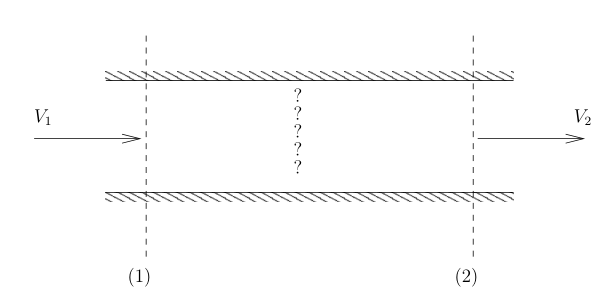
\includegraphics[width=8cm]{figures/1.png}
    \caption{正向激波}
    \label{1}
\end{figure}

\begin{align*}
    \rho_{1} V_{1} A&=\rho_{2} V_{2} A = \dot{m} \\ 
    p_{1} A+\rho_{1} A V_{1}^{2}&=p_{2} A+\rho_{2} A V_{2}^{2}\\ 
    \frac{V_{1}^{2}}{2}+\frac{\gamma}{\gamma-1} \frac{p_{1}}{\rho_{1}}&=\frac{V_{2}^{2}}{2}+\frac{\gamma}{\gamma-1} \frac{p_{2}}{\rho_{2}}
\end{align*}

对于该方程,一个非常直观的解就是$p_1=p_2,\ \rho_1=\rho_2,\ V_1=V_2$.

但除此之外,利用动量式除以质量式,代入能量式,并利用理想气体状态方程,可以得到一个非平凡的解:

\begin{align*}
    \frac{p_{2}}{p_{1}}-1&=\frac{2 \gamma}{\gamma+1}\left(M_{1}^{2}-1\right)\\ 
    \frac{\rho_{2}}{\rho_{1}}-1&=\frac{M_{1}^{2}-1}{1+\frac{\gamma-1}{2} M_{1}^{2}}\\ 
    \frac{T_{2}}{T_{1}}&=\frac{\left(2 \gamma M_{1}^{2}-(\gamma-1)\right)\left(2+(\gamma-1) M_{1}^{2}\right)}{(\gamma+1)^{2} M_{1}^{2}}\\ 
    \frac{T_{2}}{T_{1}}-1&=\frac{2(\gamma-1)\left(\gamma M_{1}^{2}+1\right)\left(M_{1}^{2}-1\right)}{(\gamma+1)^{2} M_{1}^{2}}
\end{align*}

\subsection{导管内的熵变}

\begin{align*}
    Tds&=du+pdv\\ 
    dh&=du+pdv\\ 
    v&=\frac{1}{\rho}\\ 
    ds&=c_p\frac{dT}{T}-R\frac{dp}{p}\\ 
    s_2-s_1&=c_p\ln\left(\frac{T_2}{T_1}\right)-R\ln\left(\frac{p_2}{p_1}\right)=\ln\left[\left(\frac{T_2}{T_1}\right)^{c_p}\left(\frac{p_1}{p_2}\right)^R\right]\\ 
    \frac{s_2-s_1}{c_v}&=\ln\left[\left(\frac{T_2}{T_1}^\gamma\right)\left(\frac{p_1}{p_2}\right)^{\gamma-1}\right]=\ln\left[\left(\frac{\rho_1}{\rho_2}\right)^\gamma\left(\frac{p_2}{p_1}\right)\right]
\end{align*}

代入上一节中关于压力比与密度比的式子,并且定义$m=M_1^2-1$,最终我们可以得到

\begin{equation*}
    \frac{s_{2}-s_{1}}{c_{v}}=\ln \left\{\left[\frac{(m+1)(\gamma-1)+2}{(m+1)(\gamma+1)}\right]^{\gamma}\left[1+\frac{2 \gamma m}{\gamma+1}\right]\right\}=f(m)
\end{equation*}

可以发现,导管内的熵变只与上游马赫数以及绝热指数相关。导管内的熵变可以用两部分来表示,

\begin{equation*}
    s_2-s_1=\Delta s_q+\Delta s_{irr}
\end{equation*}

其中第一项为传热带来的熵变,第二项为不可逆过程带来的熵变。如果考虑绝热流,那么根据热力学第二定律,我们可以得到

\begin{equation*}
    s_2-s_1\geq 0
\end{equation*}

从而

\begin{align*}
    M_1^2-1&\geq 0\\ 
    M_1^2&\geq 0\\ 
    \frac{p_{2}}{p_{1}} \geq 1\\ 
    \frac{\rho_{2}}{\rho_{1}} \geq 1\\ 
    \frac{V_{2}}{V_{1}} \leq 1\\ 
    \frac{T_{2}}{T_{1}} \geq 1\\ 
    \frac{T_{0_{2}}}{T_{0_{1}}}=1
\end{align*}

因此,如果等截面导管内的流体存在熵变,或是流体状态发生改变,那么入口处的流体必须是超音速的。

\subsection{正向激波内的马赫数变化}

仍然从质量守恒(连续性)方程出发,将流速用马赫数替代,并代入理想气体状态方程、声速定义和压力比、密度比关系,可以得到

\begin{align*}
    M_{2}^{2}=\frac{2+(\gamma-1) M_{1}^{2}}{2 \gamma M_{1}^{2}-\gamma+1}\\ 
    M_{2}^{2}-1=\frac{\frac{\gamma+1}{2}\left(1-M_{1}^{2}\right)}{\gamma\left(M_{1}^{2}-1\right)+\frac{\gamma+1}{2}}
\end{align*}

从而,我们得到了出口、入口马赫数$M_2\ M_1$间的关系。如图\ref{2}所示。

\begin{figure}[!ht]
    \centering
    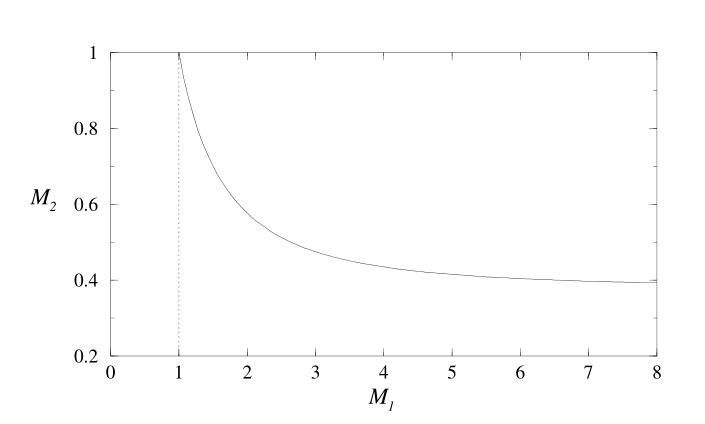
\includegraphics[width=8cm]{figures/2.png}
    \caption{出口、入口马赫数关系}
    \label{2}
\end{figure}

可以看出,入口处为超音速流体,出口处则为亚音速流体。因此可以得出结论:超音速流在经历激波后,变为亚音速流。

\subsection{弱激波下的熵增}

弱激波定义为

\begin{equation*}
    \frac{p_{2}}{p_{1}} \approx 1
\end{equation*}

不难得到,在此条件下的入口马赫数接近$1$。同时由于$m=M_1^2-1\rightarrow0$,因此

\begin{equation*}
    f(m) \approx \frac{1}{15} m^{3}
\end{equation*}

\subsection{滞止压力在激波中的变化}

对于等熵流,我们有

\begin{equation*}
    \frac{p_{0}}{p}=\left(1+\frac{\gamma-1}{2} M^{2}\right)^{\frac{\gamma}{\gamma-1}}
\end{equation*}

但对于激波而言,这个等式并不成立,因为激波本身并不是一个等熵过程。但对于间断面前后的区域,分别有

\begin{align*}
    \frac{p_{0_{1}}}{p_{1}}&=\left(1+\frac{\gamma-1}{2} M_{1}^{2}\right)^{\frac{\gamma}{\gamma-1}}\\ 
    \frac{p_{0_{2}}}{p_{2}}=\left(1+\frac{\gamma-1}{2} M_{2}^{2}\right)^{\frac{\gamma}{\gamma-1}}\\ 
    \frac{p_{0_{2}}}{p_{0_{1}}}=\frac{p_{2}}{p_{1}}\left(\frac{1+\frac{\gamma-1}{2} M_{2}^{2}}{1+\frac{\gamma-1}{2} M_{1}^{2}}\right)^{\frac{\gamma}{\gamma-1}}
\end{align*}

可以替换式中的压力比和$M_2$,从而得到

\begin{equation*}
    \frac{p_{02}}{p_{01}}=\left(\frac{\gamma+1}{2} M_{1}^{2}\right)^{\frac{\gamma}{\gamma-1}}\left(1+\frac{\gamma-1}{2} M_{1}^{2}\right)^{\frac{-\gamma}{\gamma-1}}\left(\frac{2 \gamma}{\gamma+1} M_{1}^{2}-\frac{\gamma-1}{\gamma+1}\right)^{\frac{-1}{\gamma-1}}
\end{equation*}

由于入口处为超音速流,因此$M_1>1$,

\begin{equation*}
    \frac{p_{02}}{p_{01}}<1
\end{equation*}

可以得知,滞止压力在经历激波后将会下降,且入口处马赫数越高,压力下降越多。

\subsection{二维喷管中的流体}

\begin{equation*}
    \frac{A^{*}}{A}=\frac{\left(\frac{p}{p_{o}}\right)^{\frac{1}{\gamma}}\left(1-\left(\frac{p}{p_{o}}\right)^{\frac{\gamma-1}{\gamma}}\right)^{\frac{1}{2}}}{\left(\frac{\gamma-1}{2}\right)^{\frac{1}{2}}\left(\frac{2}{\gamma+1}\right)^{\frac{\gamma+1}{2(\gamma-1)}}}
\end{equation*}

对于一个确定的喷管,如果能够确定出口处流体是超音速流体,那么出口处的压力比$p_e/p_0$就是唯一确定的。但是事实上,出口处的压力可以被设计为任意的值,这会导致在渐扩喷管中一定会出现激波,这个过程会是不可逆的。

\begin{figure}[!ht]
    \centering
    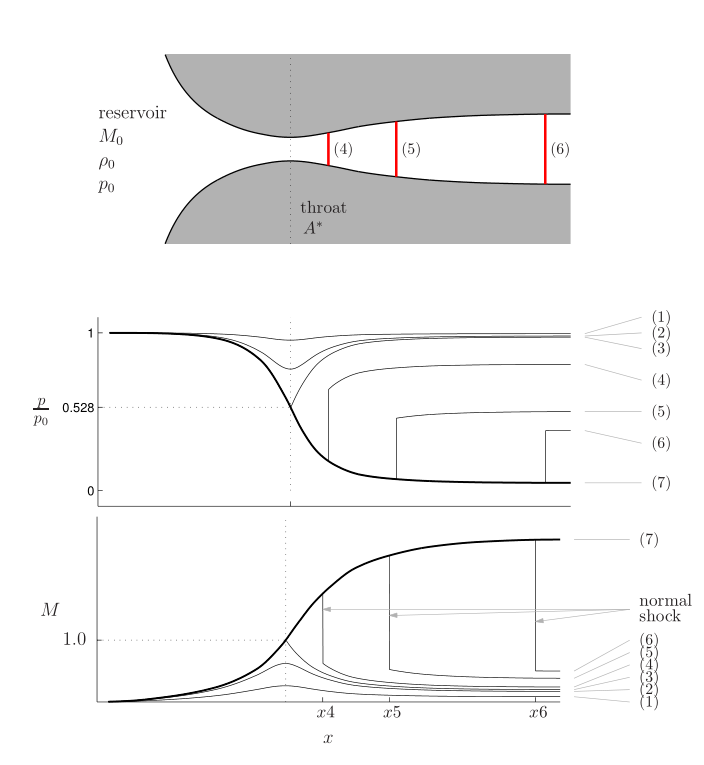
\includegraphics[width=\linewidth]{figures/3.png}
    \caption{出口压力不同导致的激波}
    \label{3}
\end{figure}

如图\ref{3}所示,分别展示了几种不同出口压力下,激波产生的位置。

\begin{itemize}
    \item (7) $p_{e7}/p_0=p_e/p_0$,全过程均为等熵流。
    \item (1),(2) 流体全程均未超过声速,同时全程均为等熵流
    \item (3) 出口压力的设置使得在喉部的流体恰好达到声速。此时,在喉部会发生弱激波,在渐扩喷管部分流体会减速,但流体全程仍为等熵流。
    \item (4) 当$p_{e4}<p_{e3}$时,流体在通过喉部之后将无法保持等熵流,因为出口压力$p_{e4}/p_0>p_{e7}/p_0$,因此一定会在渐扩喷管的某个部分发生激波。
    \item (5),(6) 与(4)类似,但由于压力比与$p_{e7}/p_0$更加接近,因此激波发生的位置也更加接近出口位置
    \item 如果压力进一步降低,斜激波将会发生
\end{itemize}

\subsection{斜激波}

考虑如图\ref{4}所示的斜激波,

\begin{figure}[!ht]
    \centering
    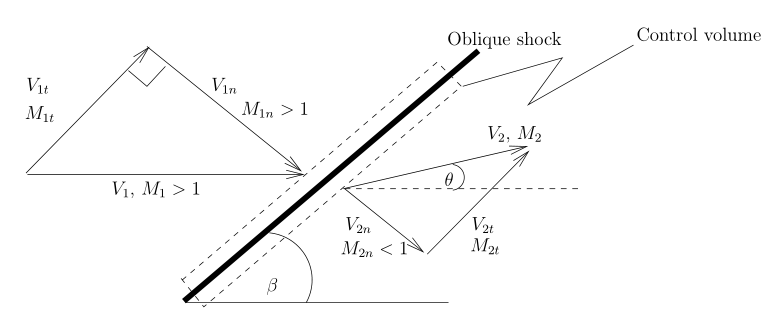
\includegraphics[width=8cm]{figures/4.png}
    \caption{斜激波}
    \label{4}
\end{figure}

考虑连续性方程与切向和法向的动量:

\begin{align*}
    \rho_{1} V_{1 n}&=\rho_{2} V_{2 n}\\ 
    p_{1}+\rho_{1} V_{1 n}^{2}&=p_{2}+\rho_{2} V_{2 n}^{2}\\ 
    \rho_{1} V_{1 n} V_{1 t}&=\rho_{2} V_{2 n} V_{2 t}
\end{align*}

不难得到$V_{1t}=V_{2t}$。由此我们可以得出,对于斜激波,在法向上,其规律与正激波一致;在切向上,速度分量则不产生变化。

如果我们基于上述结果观察一个斜激波,我们就会发现,斜激波的存在会导致流体的流向发生改变,如图\ref{5}所示。

\begin{figure}[!ht]
    \centering
    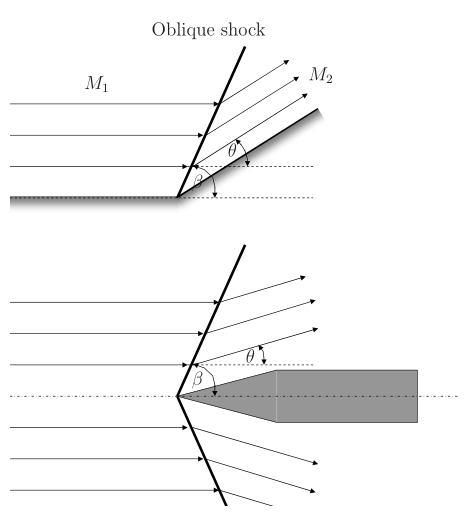
\includegraphics[width=8cm]{figures/5.png}
    \caption{斜激波导致流体流向的变化}
    \label{5}
\end{figure}

\begin{align*}
    M_{1}&=\frac{M_{1 n}}{\sin \beta}\\ 
    M_{2}&=\frac{M_{2 n}}{\sin (\beta-\theta)}
\end{align*}

注意到,$M_1>1$,但$M_{2n}<1$并不意味着$M_2<1$。在经历斜激波后,流体仍然可能是超音速的。

\subsection{马赫角}

对于超音速流体,如图\ref{6}所示的圆锥顶角称为马赫角$\mu$,

\begin{figure}[!ht]
    \centering
    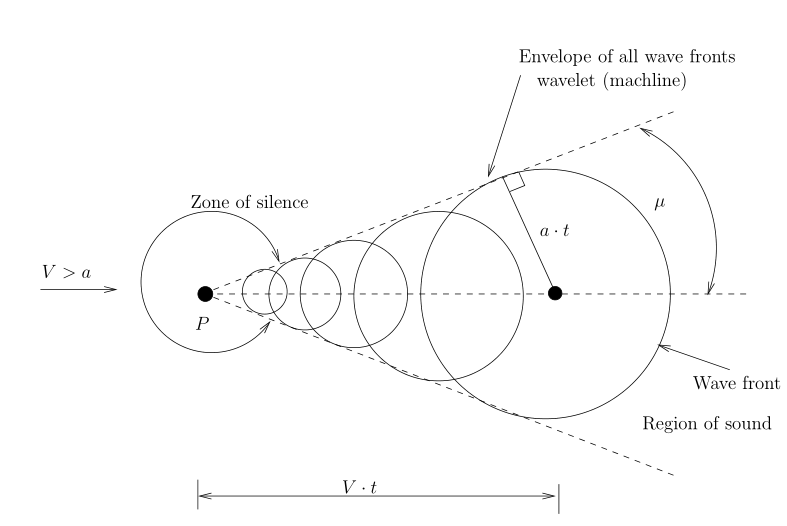
\includegraphics[width=8cm]{figures/6.png}
    \caption{马赫角}
    \label{6}
\end{figure}

满足

\begin{align*}
    \sim\mu&=\frac{a}{V}=\frac{1}{M}\\ 
    M&=\frac{1}{\sin\mu}\\ 
    \sin\mu&=\frac{1}{M}
\end{align*}

当超音速流体遇到遇到较强的物理约束时,此时斜激波就会产生,并且满足关系

\begin{equation*}
    M_{1 n}=M_{1} \sin \beta=\frac{\sin \beta}{\sin \mu}>1
\end{equation*}

斜激波的角度始终大于马赫角,$\beta>\mu$。

\subsection{偏折角$\theta$与激波倾角$\beta$间的关系}

\begin{figure}[!ht]
    \centering
    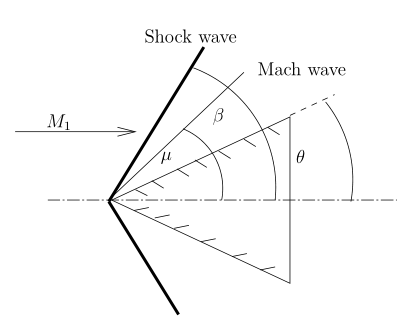
\includegraphics[width=8cm]{figures/7.png}
    \caption{偏折角与激波倾角间的关系}
    \label{7}
\end{figure}

利用之前的结论,对于斜激波,在法向上,正激波的结论依然适用,因此

\begin{equation*}
    \frac{\rho_{2}}{\rho_{1}}=\frac{\frac{\gamma+1}{2}\left(M_{1} \sin \beta\right)^{2}}{1+\frac{\gamma-1}{2}\left(M_{1} \sin \beta\right)^{2}}
\end{equation*}

考虑到激波两侧的连续性,因此

\begin{align*}
    \frac{\rho_{2}}{\rho_{1}}&=\frac{V_{1 n}}{V_{2 n}}\\ 
    &=\frac{V_{1 n}}{V_{1 t}} \frac{V_{2 t}}{V_{2 n}}\\ 
    &=\frac{\tan \beta}{\tan (\beta-\theta)}
\end{align*}

把上述两式进行比较,可以得到

\begin{align*}
    \tan \theta&=\frac{\tan \beta\left(M_{1}^{2} \sin ^{2} \beta-1\right)}{\tan ^{2} \beta \frac{\gamma}{2} M_{1}^{2}+\frac{1}{2} M_{1}^{2} \sin ^{2} \beta\left(1-\tan ^{2} \beta\right)+\tan ^{2} \beta}\\ 
    &=2 \cot \beta\left[\frac{M_{1}^{2} \sin ^{2} \beta-1}{M_{1}^{2}(\gamma+\cos 2 \beta)+2}\right]
\end{align*}

对应关系可以从图\ref{8}中得到更直观的了解。

\begin{figure}[!ht]
    \centering
    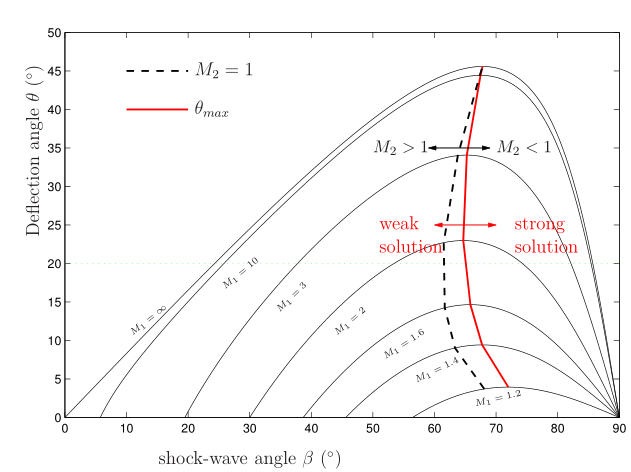
\includegraphics[width=8cm]{figures/8.png}
    \caption{$\theta$ vs. $\beta$}
    \label{8}
\end{figure}

可以看出,对于给定的$\theta$角,有两个$\beta$角与之对应,其中一个为出流马赫数小于1的强解,另一个为出流马赫数大于1的弱解。在实际中,出现的究竟是强解还是弱解,取决于背景中的压力;一般而言,弱解更加常见,但是如果提升背景压力,则强解也有可能出现。

\begin{align*}
    M_{2 \text { strong }}&<M_{2 \text { weak }}\\ 
    \beta_{\text {strong }}&>\beta_{\text {weak }}
\end{align*}

\subsection{斜激波的特殊解}

\begin{enumerate}
    \item 从喷管进入高压区域的超音速流体(喷气式飞机)
    
    当$p_{e7}<p_e<p_{e6}$时,接近出口处的流体将会是超音速流,并且在喷管出口处的压力将会与$p_{e7}$相等,但当流体到达出口处时,必须立刻提升压力到$p_e$,为了达到这样的效果,斜激波会在出口的边角处生成。

    涡流层的存在是压力发生骤变的原因。把正激波的式子代入斜激波的法向,可以得到

    \begin{equation*}
        \frac{p_{2}}{p_{1}}=\frac{2 \gamma}{\gamma+1}\left(M_{1}^{2} \sin ^{2} \beta-1\right)
    \end{equation*}

    其中$p_1$是出口前压力,$p_2$是出口后压力,通过这个式子以及已知的$M_1$,我们可以得到对应的$\beta$角,从而找到对应的$\theta$和$M_2$。

    \item 固体边界带来的激波反射
    
    当激波碰到墙时,激波也会反射,而对应的反射角由墙带来的边界条件确定:原本平行于墙面的流体在经过激波的两次折射后,仍然平行于墙面,如图\ref{9}所示。

    \begin{figure}[!ht]
        \centering
        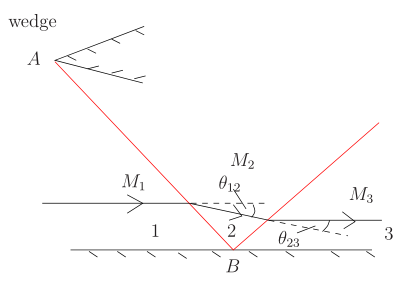
\includegraphics[width=8cm]{figures/9.png}
        \caption{激波的反射}
        \label{9}
    \end{figure}
\end{enumerate}

\subsection{马赫线与其性质}

通过马赫线,如果气体被压缩,则马赫数减小,马赫角增加;若通过马赫线,气体膨胀,则马赫数增加,马赫角减小。

\begin{enumerate}
    \item 凹角

    \begin{figure}[!ht]
        \centering
        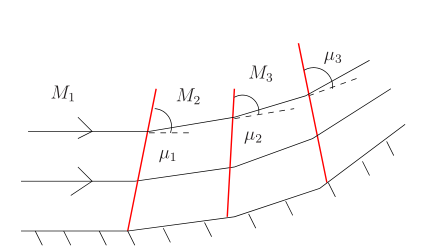
\includegraphics[width=8cm]{figures/10.png}
        \caption{凹角马赫线}
        \label{10}
    \end{figure}

    如图\ref{10}所示,凹角处存在一系列压缩的马赫线,$M_1>M_2>M_3$,$\mu_1<\mu_2<\mu_3$。通过马赫线的流体可以视为等熵流。同时如图\ref{11},这一系列的马赫线会交汇于一点,此时,激波生成了。同时,在这个交汇点的后方,也存在一个涡流层,涡流层上下流体的速度是不连续的,但压力仍然是连续的。在涡流层和固体边界之间的流体可以视为等熵流提,他们只经过了一系列马赫线;在涡流层上方的流体通过了激波间断线,因为通过了斜激波,存在熵变,因此不可逆,等熵关系不再保持。

    \begin{figure}[!ht]
        \centering
        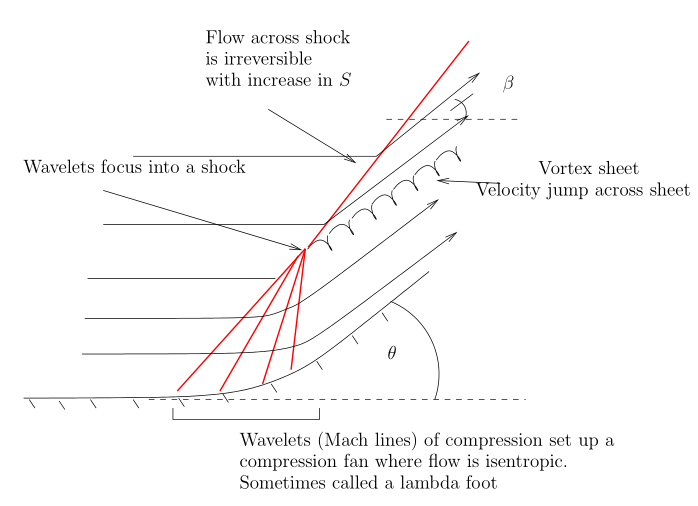
\includegraphics[width=8cm]{figures/11.png}
        \caption{凹角处的激波}
        \label{11}
    \end{figure}

    \begin{align*}
        \frac{T_{0}}{T}&=1+\frac{\gamma-1}{2} M^{2}\quad\mbox{对所有流体适用}\\ 
        \frac{p_{0}}{p}&=\left(1+\frac{\gamma-1}{2} M^{2}\right)^{\frac{\gamma}{\gamma-1}}\quad\mbox{仅对绝热流体适用}\\ 
        \frac{\rho_{0}}{\rho}=\left(1+\frac{\gamma-1}{2} M^{2}\right)^{\frac{1}{\gamma-1}}\quad\mbox{仅对绝热流体适用}
    \end{align*}

    \item 凸角
    
    对于凸角,同样存在一系列扩张马赫线,如图\ref{12}所示,$M_1<M_2<M_3$,$\mu_1>\mu_2>\mu_3$。但是这一系列的扩张马赫线并不会汇聚于一点。在凸角处,这一现象被称为Prantdl-Meyer膨胀扇,如图\ref{13}。在这种条件下,整个流体都是等熵的。


    \begin{figure}[!ht]
        \centering
        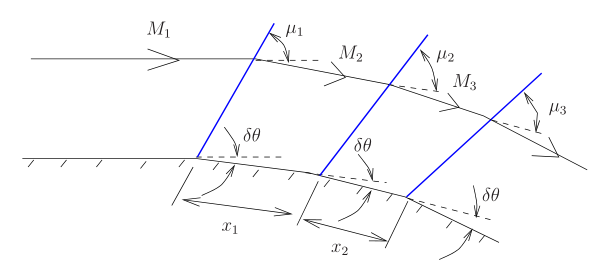
\includegraphics[width=8cm]{figures/12.png}
        \caption{凸角马赫线}
        \label{12}
    \end{figure}

    
    \begin{figure}[!ht]
        \centering
        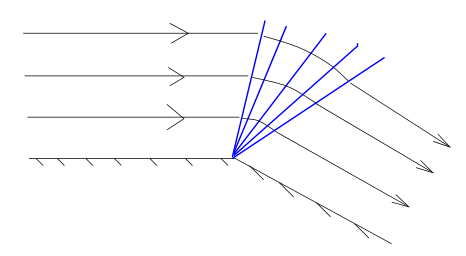
\includegraphics[width=8cm]{figures/13.png}
        \caption{凸角马赫线}
        \label{13}
    \end{figure}
\end{enumerate}

\subsection{马赫线分析}

考虑如图\ref{14}所示的凹角,对控制体分析:

\begin{figure}[!ht]
    \centering
    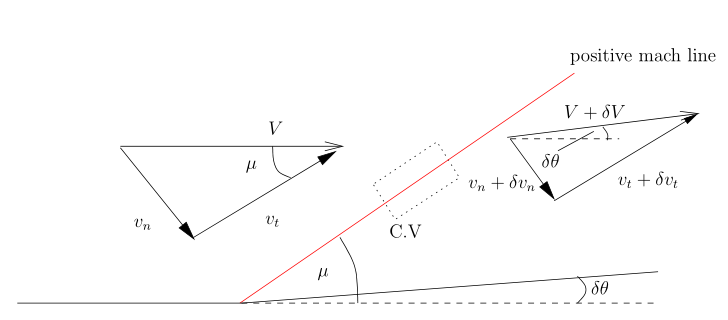
\includegraphics[width=\linewidth]{figures/14.png}
    \caption{马赫线分析}
    \label{14}
\end{figure}

质量守恒

\begin{align*}
    \rho v_n&=(\rho+\delta\rho)(v_n+\delta v_n)\\ 
    0&=v_n\delta\rho+\rho\delta v_n
\end{align*}

切向方向的动量守恒

\begin{align*}
    \rho v_{n} v_{t}&=(\rho+\delta \rho)\left(v_{n}+\delta v_{n}\right)\left(v_{t}+\delta v_{t}\right)\\ 
    \delta v_{t}&=0
\end{align*}

也可以写作

\begin{equation*}
    V\cos\mu=(V+\delta V)\cos(\mu-\delta\theta)
\end{equation*}

利用和角公式,并近似$\sin\delta\theta\rightarrow\delta\theta$,$\cos\delta\theta\rightarrow1$,可以得到

\begin{equation*}
    V \cos \mu=(V+\delta V)(\cos \mu+\delta \theta \sin \mu)
\end{equation*}

展开并忽略高阶小量,可以得到

\begin{align*}
    \delta V \cot \mu&=-V \delta \theta\\ 
    \delta \theta&=\mp \frac{\delta V}{V} \sqrt{M^{2}-1}
\end{align*}

式中的$\mp$代表,对于正的马赫线,此处取负号;对于负的马赫线,此处取正号。

为了将$\theta$与压力变化$\delta p$联系起来,利用欧拉方程:

\begin{equation*}
    \int \frac{d p}{\rho}+\frac{V^{2}}{2}=\mathrm{const}
\end{equation*}

微分得到

\begin{equation*}
    \frac{\delta p}{\rho}=-V \delta V
\end{equation*}

代回前式可得

\begin{align*}
    \delta \theta&=\pm \frac{\delta p}{\rho V^{2}} \sqrt{M^{2}-1}\\ 
    &=\pm \frac{\delta p}{\gamma p M^{2}} \sqrt{M^{2}-1}\\ 
    &=\mp \frac{\delta M\left(M^{2}-1\right)^{\frac{1}{2}}}{M\left(1+\frac{M^{2}(\gamma-1)}{2}\right)}
\end{align*}

对于上式进行积分,

\begin{align*}
    \theta&=\mp \int \frac{d M\left(M^{2}-1\right)^{\frac{1}{2}}}{M\left(1+\frac{M^{2}(\gamma-1)}{2}\right)}\\ 
    &=\mp \omega(M)+\theta_{0}
\end{align*}

其中$\omega(M)$被称为Prandtl角,为积分

\begin{equation*}
    \omega(M)=[\sqrt{\frac{\gamma+1}{\gamma-1}} \arctan \sqrt{\frac{\gamma-1}{\gamma+1}\left(M^{2}-1\right)}-\arctan \sqrt{M^{2}-1}]
\end{equation*}

也可以通过查表得到。

因此,我们有结论

\begin{equation*}
    \theta\pm\omega(M)=\theta_0=\mathrm{const}
\end{equation*}

对于流体的全过程成立。

马赫线与偏转角度的正负定义如图\ref{15}所示。注意到,$\mu=\arcsin(1/M)$,始终是正值。

\begin{figure}[!ht]
    \centering
    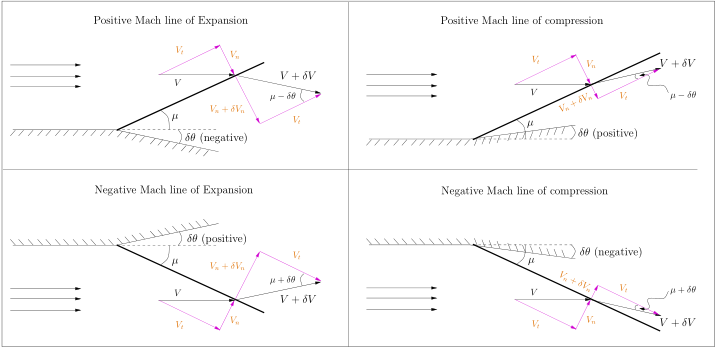
\includegraphics[width=\linewidth]{figures/15.png}
    \caption{马赫线与偏转角度的正负定义}
    \label{15}
\end{figure}

从而,

\begin{align*}
    V \cos \mu&=(V+\delta V) \cos (\mu-\delta \theta)\quad\mbox{正马赫线}\\ 
    V \cos \mu&=(V+\delta V) \cos (\mu+\delta \theta)\quad\mbox{负马赫线}
\end{align*}

\begin{equation*}
    \delta \theta=\mp \frac{\sqrt{M^{2}-1}}{M\left(1+\frac{\gamma-1}{2} M^{2}\right)} \delta M
\end{equation*}
\section{数学}

\subsection{高斯散度定理}

\begin{equation*}
    \iiint_{\Omega} \operatorname{div} \mathbf{A} d v=\oiint_{\Sigma} \mathbf{A} \cdot \mathbf{n} d S
\end{equation*}

其中$\Sigma$是空间闭区域$\Omega$的边界,$\mathbf{n}$为曲面$\Sigma$朝外的单位向量。



\end{document}